\chapter{Desenvolvimento}
\label{cap:desenvolvimento}
\textcolor{red}{[PENDENTE: parágrafo de abertura do capítulo]}


\section{RISC-V}
\label{sec:risc-v}

As intrunçoes do conjunto RV32I são organizado dentro dos quattros formatos basicos exibidos na Figura \ref{fig:formatoInstrucaoRV32I_2}, porem para alguns cassos esses formatos puros não são suficiente para conteplar todas posibilidades, ou não são o mais eficiente, por causa disso exite algumas variçoes,  

\begin{figure}[!htb]%% Ambiente figure
     \centering % Centraliza a imagem no documento (recomendado)
     \caption{Formato das instruções da RV32I}% Legenda da sua figura
     \label{fig:formatoInstrucaoRV32I_2}%rotulo
     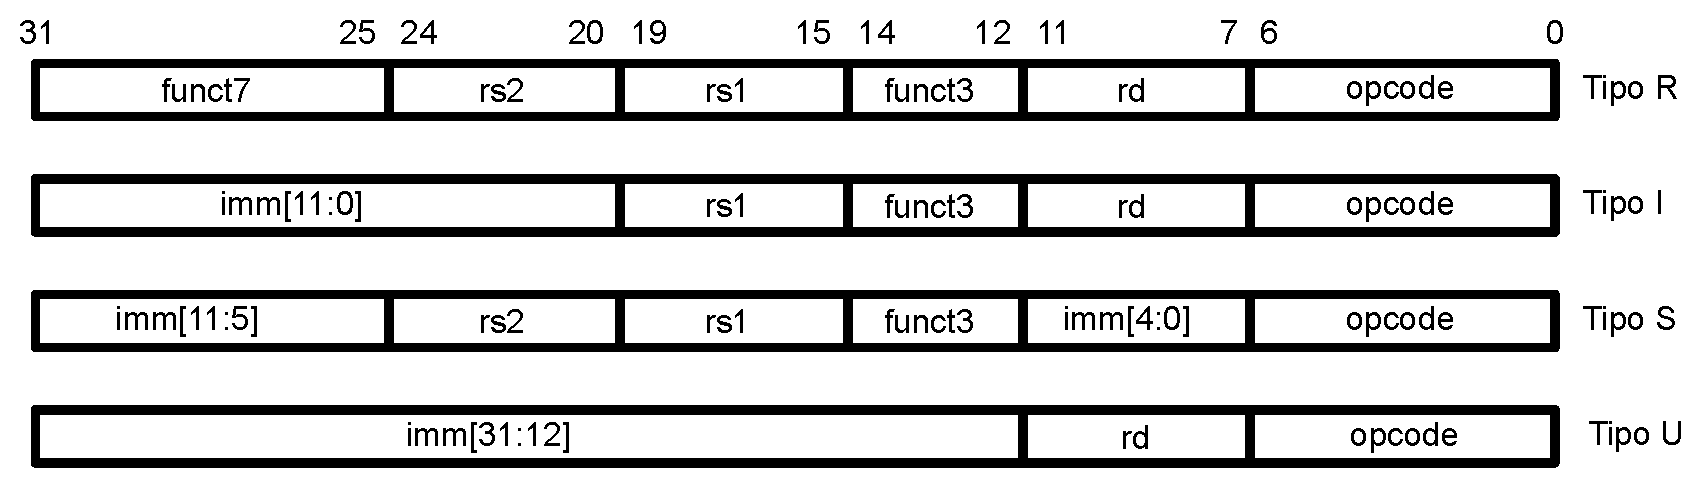
\includegraphics[scale=0.54]{figuras/instrucaoRISC-V.pdf}
     \fonte{Adaptado de \cite{riscv_manual_2026}}%% Fonte adaptada
\end{figure}

Dentro do conjunto RV32I as instruções são dividas em cinco categoraias: Inteiros, Transferência de controle, Carga e Descarga da memoria, Ordenação da memoria e Chamada de ambiente \cite{riscv_manual_2026}.

O conjunto dos inteiros é composto por 21 intruçoes e é o resposalvel por realizar as operaçoes matemticas soma e subtração, e operaçoes logicas de comapração, deslocamento, AND, OR ou XOR. A operação pode ser realizada tanto entre dois numeros vindo de registradores, quanto entre um registrador e um valor constante vindo diretemente da intrução que é nomeado de imediato.

% NOTA (Overleaf, 09/09): "Ver se vou implementar a instrução, se não vira uma NOP".
% Resolvido no RTL: ECALL, EBREAK e FENCE viram NOP, sem trap (37 instruções executadas). Texto abaixo ainda fala em trap e em 38.
O conjunto RV32I possui originalmente 40 instruções em sua especificação base; contudo, implementações simples como a proposta neste trabalho podem reduzir para 38 intruçoes. A primeira redução ocorre nas duas únicas instruções do tipo SYSTEM: a instrução \texttt{ECALL}, responsável por solicitar chamadas de sistema (\textit{system calls}) ao sistema operacional, e a instrução \texttt{EBREAK}, utilizada por depuradores para pausar a execução do programa e devolver o controle ao ambiente de desenvolvimento. Em um núcleo de ciclo único sem suporte a sistema operacional ou depuração em tempo real, ambas as instruções podem ser unificadas em uma rotina simplificada de exceção (\textit{trap}), disparando um sinal de interrupção ou paralisando a execução do circuito de forma controlada \cite{riscv_manual_2026}. 


Outra instrução que pode ser simplificada em implementações de escopo reduzido é a \texttt{FENCE}. Essa instrução é responsável por garantir o ordenamento na execução de memória em sistemas multicore ou em microarquiteturas avançadas com execução fora de ordem (\textit{out-of-order}). Como o processador projetado neste trabalho é de núcleo único e possui execução estritamente sequencial em ciclo único, a ordenação das operações de memória é garantida nativamente pela própria estrutura física. Dessa forma, a instrução \texttt{FENCE} torna-se redundante, podendo ser tratada funcionalmente como uma instrução NOP (do inglês \textit{No Operation}), isto é, uma operação nula que não altera o estado dos registradores nem da memória \cite{riscv_manual_2026}.

